\documentclass[aspectratio=169,11pt]{beamer}

\usetheme{default}
\usecolortheme{default}
\setbeamertemplate{navigation symbols}{}

\definecolor{nyupurple}{RGB}{87,35,100}
\definecolor{darkblue}{RGB}{0,40,85}
\definecolor{lightgray}{RGB}{245,245,245}
\definecolor{darkgray}{RGB}{64,64,64}

\setbeamercolor{frametitle}{fg=white,bg=darkblue}
\setbeamercolor{title}{fg=darkblue}
\setbeamercolor{author}{fg=black}
\setbeamercolor{institute}{fg=black}
\setbeamercolor{date}{fg=black}
\setbeamercolor{structure}{fg=darkblue}
\setbeamercolor{normal text}{fg=black}
\setbeamercolor{itemize item}{fg=nyupurple}
\setbeamercolor{itemize subitem}{fg=darkblue}
\setbeamercolor{enumerate item}{fg=darkblue}

\newlength{\titlebandht}
\setlength{\titlebandht}{4ex}
\setbeamertemplate{frametitle}{
  \nointerlineskip
  \begin{beamercolorbox}[wd=\paperwidth,ht=\titlebandht,dp=1.1ex,leftskip=1.2em,rightskip=1.2em]{frametitle}
    \usebeamerfont{frametitle}\insertframetitle
    \ifx\insertframesubtitle\@empty\relax\else\\[-0.2ex]
      \usebeamerfont{framesubtitle}\insertframesubtitle
    \fi
  \end{beamercolorbox}
  \vspace{0.6em}
}
\setbeamertemplate{footline}{\hfill\insertframenumber\hspace{2em}\vspace{0.5em}}

\usefonttheme{professionalfonts}
\usefonttheme{serif}

\usepackage{amsmath,amssymb,amsthm}
\usepackage{graphicx}
\usepackage{booktabs}
\usepackage{adjustbox}
\usepackage{mathtools}
\usepackage{bm}
\usepackage{bbm}

\newcommand{\E}{\mathbb{E}}
\renewcommand{\P}{\mathbb{P}}
\newcommand{\R}{\mathbb{R}}
\newcommand{\Cov}{\text{Cov}}
\newcommand{\Var}{\text{Var}}
\DeclareMathOperator*{\argmin}{arg\,min}
\DeclareMathOperator*{\argmax}{arg\,max}

\setbeamercolor{block title}{bg=lightgray,fg=darkblue}
\setbeamercolor{block body}{bg=lightgray!50}
\setbeamercolor{block title alerted}{bg=nyupurple!15,fg=nyupurple}
\setbeamercolor{block body alerted}{bg=nyupurple!5}

\graphicspath{{../tex/}}

\title{Problem Set 3: Income Fluctuations and Ergodic Distributions}
\subtitle{Solutions + Comments}
\author{Rafael Lincoln}
\institute{New York University}
\date{\today}

\begin{document}

% ============================================================================
% SLIDE 1: TITLE
% ============================================================================
\begin{frame}[plain]
    \titlepage
\end{frame}

% ============================================================================
% SLIDE 2: ROADMAP
% ============================================================================
\begin{frame}{Roadmap}
    \begin{columns}[T]
        \begin{column}{0.48\textwidth}
            \textbf{Problem 1: Two-State Income}
            \begin{itemize}\setlength\itemsep{0.2em}
                \item Discrete (employed/unemployed) income
                \item Three solution methods: Grid VFI, Coefficient VFI, Howard
                \item Ergodic distribution via transition matrix eigenvector
            \end{itemize}
        \end{column}
        \begin{column}{0.48\textwidth}
            \textbf{Problem 2: AR(1) Income}
            \begin{itemize}\setlength\itemsep{0.2em}
                \item Continuous income, Gaussian quadrature expectations
                \item Tensor-product spline collocation on Greville nodes
                \item Decision rules, Euler diagnostics, ergodic distribution
            \end{itemize}
        \end{column}
    \end{columns}
    \vspace{0.5em}
    \begin{alertblock}{Common thread}
        \small Both problems illustrate the gap between \textbf{solve grid} (where the Bellman is enforced) and \textbf{output grid} (where distributions and moments are computed).
    \end{alertblock}
\end{frame}

% ============================================================================
%  PROBLEM 1
% ============================================================================

% ============================================================================
% SLIDE 3: P1 -- ECONOMIC ENVIRONMENT
% ============================================================================
\begin{frame}{Problem 1: Economic Environment}
    \textbf{Household problem} with two income states $e \in \{\text{employed},\text{unemployed}\}$:
    \[
    \begin{aligned}
    E(a) &= \max_{a'\ge 0}\; \log\bigl((1+r)a + 1 - a'\bigr) + \beta\bigl[(1-\sigma)E(a') + \sigma U(a')\bigr] \\[3pt]
    U(a) &= \max_{a'\ge 0}\; \log\bigl((1+r)a + b - a'\bigr) + \beta\bigl[\lambda E(a') + (1-\lambda)U(a')\bigr]
    \end{aligned}
    \]

    \vspace{0.3em}
    \begin{columns}[T]
        \begin{column}{0.46\textwidth}
            \textbf{Income and transitions}
            \begin{itemize}\setlength\itemsep{0.1em}
                \item Employed: $y=1$, Unemployed: $y=b=0.25$
                \item $\sigma=0.10$ (job-loss rate)
                \item $\lambda=0.25$ (job-finding rate)
                \item Fraction employed: $\lambda/(\sigma+\lambda)=0.714$
            \end{itemize}
        \end{column}
        \begin{column}{0.50\textwidth}
            \textbf{Calibration and grid}
            \begin{itemize}\setlength\itemsep{0.1em}
                \item $\beta=0.95$, $r=0.04$, $a\in[0,10]$
                \item Borrowing constraint: $a'\ge 0$
                \item 51 cubic spline breakpoints; 53 Greville collocation nodes
                \item Dense evaluation grid: 551 pts (quadratic spacing)
            \end{itemize}
        \end{column}
    \end{columns}
\end{frame}

% ============================================================================
% SLIDE 4: P1 -- SOLUTION METHODS AND CONVERGENCE
% ============================================================================
\begin{frame}{Problem 1: Solution Methods and Convergence}
    \textbf{Three methods} solving the same fixed point:

    \begin{itemize}\setlength\itemsep{0.2em}
        \item \textbf{Grid VFI}: maximize Bellman at each of 551 grid points via golden-section search; interpolate continuation value with cubic spline.
        \item \textbf{Coefficient VFI}: represent $E(\cdot)$, $U(\cdot)$ as spline coefficients $\theta_e$, $\theta_u$; update $\theta^{t+1} = \Phi^{-1} v^t$ at each iteration.
        \item \textbf{Howard Improvement}: fix policy $a'(a)$; solve the \textbf{linear system} for coefficients directly; repeat until policy stabilizes.
    \end{itemize}

    \vspace{0.4em}
    \begin{center}
    \small
    \renewcommand{\arraystretch}{1.15}
    \begin{tabular}{lccc}
        \toprule
        \textbf{Method} & \textbf{Iterations} & \textbf{Final error} & \textbf{Max $\Delta$ value vs Grid} \\
        \midrule
        Grid VFI & 336 & \texttt{9.70e-09} & --- (benchmark) \\
        Coefficient VFI & 420 & \texttt{9.50e-10} & \texttt{2.19e-04} \\
        Howard & \textbf{7} & \texttt{2.76e-14} & \texttt{2.19e-04} \\
        \bottomrule
    \end{tabular}
    \end{center}
    \vspace{0.2em}
    \footnotesize
    Max absolute difference in savings policy (employed): \texttt{1.22e-03} for both Coefficient VFI and Howard.
\end{frame}

% ============================================================================
% SLIDE 5: P1 -- VALUE FUNCTIONS AND SAVINGS POLICIES
% ============================================================================
\begin{frame}{Problem 1: Value Functions and Savings Policies}
    \vspace{-0.6em}
    \begin{center}
        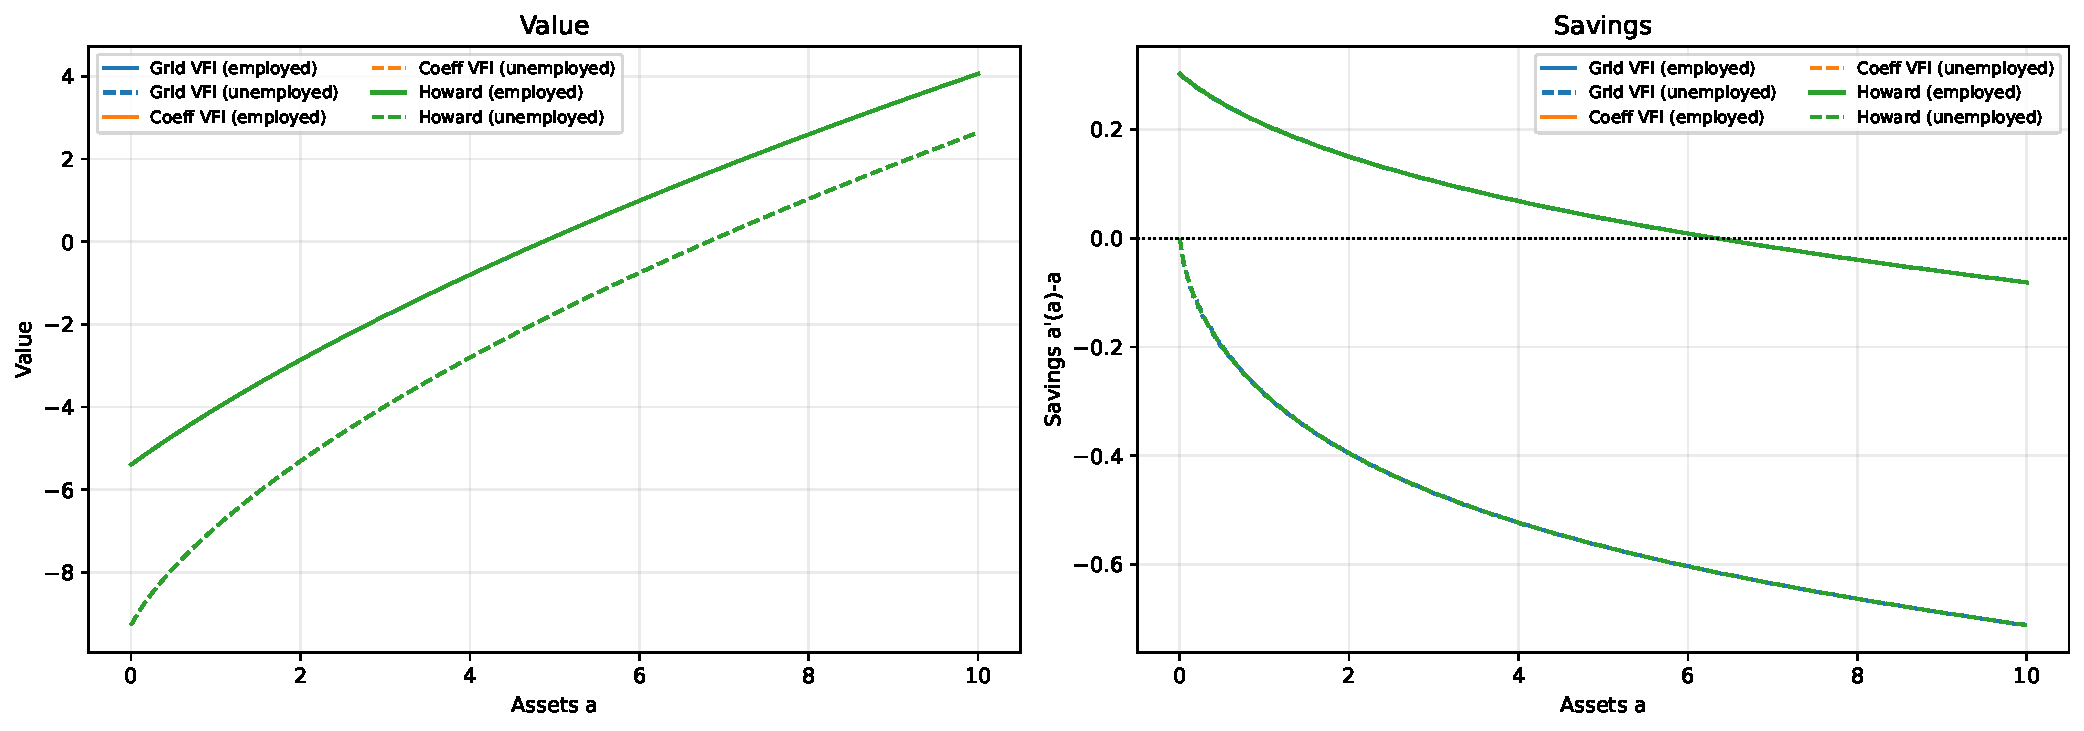
\includegraphics[width=0.92\textwidth]{fig_p1_value_and_savings.pdf}
    \end{center}
    \vspace{-0.5em}
    \small
    \textbf{Left}: Value functions $E(a)$ and $U(a)$ — all three methods overlap perfectly (max diff $\sim 2\times10^{-4}$). \quad
    \textbf{Right}: Net savings $a'(a)-a$ — employed agents save more at every wealth level; the zero-crossing identifies the \textbf{target wealth}. Both states show a region of dis-saving near the borrowing constraint.
\end{frame}

% ============================================================================
% SLIDE 6: P1 -- ERGODIC DISTRIBUTION
% ============================================================================
\begin{frame}{Problem 1: Ergodic Distribution}
    \vspace{-0.4em}
    \begin{columns}[T]
        \begin{column}{0.58\textwidth}
            \begin{center}
                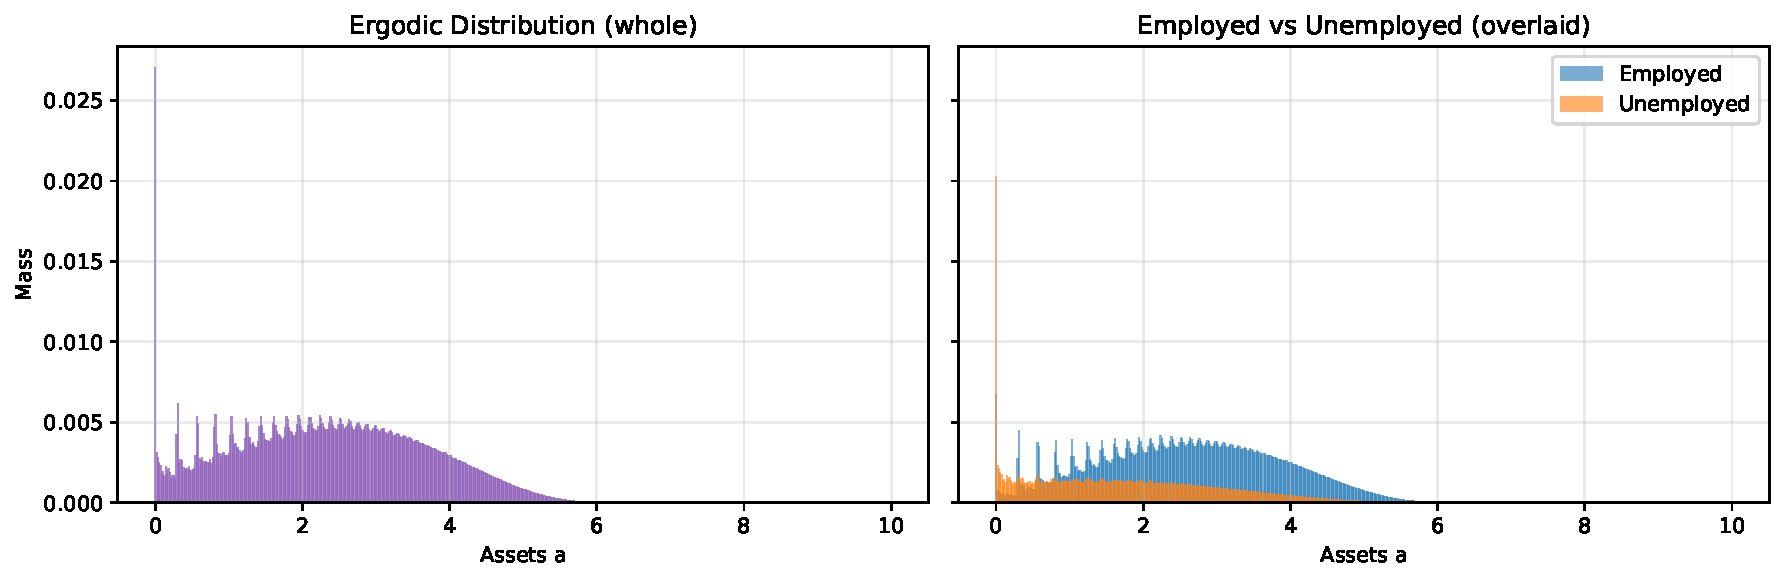
\includegraphics[width=\linewidth]{fig_p1_ergodic_dist.pdf}
            \end{center}
        \end{column}
        \begin{column}{0.38\textwidth}
            \footnotesize
            \textbf{Method}: Transition matrix $Q$ from spline basis; stationary eigenvector (unit eigenvalue).

            \vspace{0.4em}
            \textbf{Ergodic moments}\\[0.3em]
            \renewcommand{\arraystretch}{1.1}
            \begin{tabular}{lc}
                \toprule
                & Value \\
                \midrule
                Fraction employed & 0.714 \\
                Mean assets (E) & 2.60 \\
                Mean assets (U) & 1.75 \\
                Mean consump.\ (E) & 0.97 \\
                Mean consump.\ (U) & 0.65 \\
                Stationarity error & \texttt{1.3e-17} \\
                \bottomrule
            \end{tabular}

            \par\vspace{0.4em}
            {\sloppy\textbf{Takeaway}: Unemployed agents hold \textit{less} wealth on average --- precautionary savings collapse near the borrowing constraint.\par}
        \end{column}
    \end{columns}
\end{frame}

% ============================================================================
%  PROBLEM 2
% ============================================================================

% ============================================================================
% SLIDE 7: P2 -- ECONOMIC ENVIRONMENT
% ============================================================================
\begin{frame}{Problem 2: Continuous AR(1) Income --- Environment}
    \textbf{Household Bellman equation}:
    \[
    \boxed{
    V(a,z) = \max_{a'\ge 0}\; \frac{c^{1-\alpha}}{1-\alpha} + \beta \int V(a',\rho z + \sigma\varepsilon')\,dF(\varepsilon')
    \quad\text{s.t.}\quad c + a' = e^z + (1+r)a
    }
    \]

    \vspace{0.3em}
    \begin{columns}[T]
        \begin{column}{0.46\textwidth}
            \textbf{Income process}
            \begin{itemize}\setlength\itemsep{0.1em}
                \item AR(1) in logs: $z_{t+1} = \rho z_t + \sigma\varepsilon_{t+1}$, $\varepsilon\sim\mathcal{N}(0,1)$
                \item $\rho=0.90$, $\sigma=0.20$
                \item $z$ grid: $\pm 4\,\sigma_z^{\infty}$ from mean, $\sigma_z^\infty = \sigma/\sqrt{1-\rho^2}$
                \item Expectations: Gauss--Hermite quadrature ($k=7$ nodes)
            \end{itemize}
        \end{column}
        \begin{column}{0.50\textwidth}
            \textbf{Calibration}
            \begin{itemize}\setlength\itemsep{0.1em}
                \item $\beta=0.95$, $r=0.02$, $\alpha=1.5$ (CRRA)
                \item $a \in [0,50]$, 51 breakpoints ($u^2$ spacing)
                \item 15 $z$ breakpoints, total \textbf{901 collocation nodes}
                \item Greville abscissae as solve grid; dense uniform grid for output
            \end{itemize}
        \end{column}
    \end{columns}
\end{frame}

% ============================================================================
% SLIDE 8: P2 -- GRID DESIGN AND SOLVE VS OUTPUT
% ============================================================================
\begin{frame}[shrink=8]{Problem 2: Grid Design --- Solve Grid vs.\ Output Grid}
    \vspace{-0.2em}
    \begin{columns}[T]
        \begin{column}{0.52\textwidth}
            \small\textbf{Asset grid ($a$-axis):} 51 breakpoints via $u^2$ clustering $\Rightarrow$ 53 Greville nodes. Dense coverage at low $a$.

            \vspace{0.2em}
            \small\textbf{Income grid ($z$-axis):} 15 breakpoints $\Rightarrow$ 17 Greville nodes. Range: $\pm 4\,\sigma_z^\infty$.

            \vspace{0.2em}
            \small\textbf{Total:} $53\!\times\!17 = 901$ collocation states where the Bellman is solved.
        \end{column}
        \begin{column}{0.44\textwidth}
            \begin{alertblock}{Key distinction}
                \small
                \textbf{Solve grid}: Greville nodes (901 pts). Bellman enforced \textit{only} here; spacing set by the spline basis.

                \vspace{0.15em}
                \textbf{Output grid}: dense uniform grid (e.g.\ $101\!\times\!31$) for distribution, moments, and Euler diagnostics. Policies \textit{evaluated} here via spline.

                \vspace{0.15em}
                Mixing the two is the most common source of distribution errors.
            \end{alertblock}
        \end{column}
    \end{columns}
\end{frame}

% ============================================================================
% SLIDE 9: P2 -- SOLUTION METHODS AND CONVERGENCE
% ============================================================================
\begin{frame}{Problem 2: Solution Methods and Convergence}
    \textbf{Coefficient VFI}: solve $\theta^{t+1} = \Phi^{-1} v(a,z;\theta^t)$ at 901 collocation nodes.

    \vspace{0.3em}
    \textbf{Howard}: fix optimal policy; update $\theta$ by solving the linear system
    \[
    \bigl[\Phi - \beta\textstyle\sum_{k=1}^K w_k \Phi(a'(\cdot), \rho z + \sigma\varepsilon_k)\bigr]\,\theta = u(c)
    \]
    until coefficients converge; then recompute policy.

    \vspace{0.4em}
    \begin{center}
    \footnotesize
    \renewcommand{\arraystretch}{1.15}
    \begin{tabular}{lcccr}
        \toprule
        \textbf{Method} & \textbf{Iter} & \textbf{Error} & \textbf{Time} & \textbf{$\Delta V$ vs Grid} \\
        \midrule
        Grid VFI ($81\!\times\!25$) & 285 & \texttt{9.56e-07} & 2.6\,s & benchmark \\
        Coeff VFI (901 nodes) & 285 & \texttt{9.56e-07} & 45\,s & $<$\texttt{1e-04} \\
        Howard (901 nodes) & \textbf{6} & \texttt{2.27e-08} & fast & $<$\texttt{1e-04} \\
        \bottomrule
    \end{tabular}
    \end{center}
    \par\vspace{0.2em}
    {\footnotesize\sloppy\textbf{Takeaway}: Howard: 6 iterations vs.\ 285 (VFI). Same fixed point; far fewer maximization calls.\par}
\end{frame}

% ============================================================================
% SLIDE 10: P2 -- 3D POLICY SURFACES
% ============================================================================
\begin{frame}{Problem 2: Policy Surfaces (Howard Solution)}
    \vspace{-0.3em}
    \begin{center}
        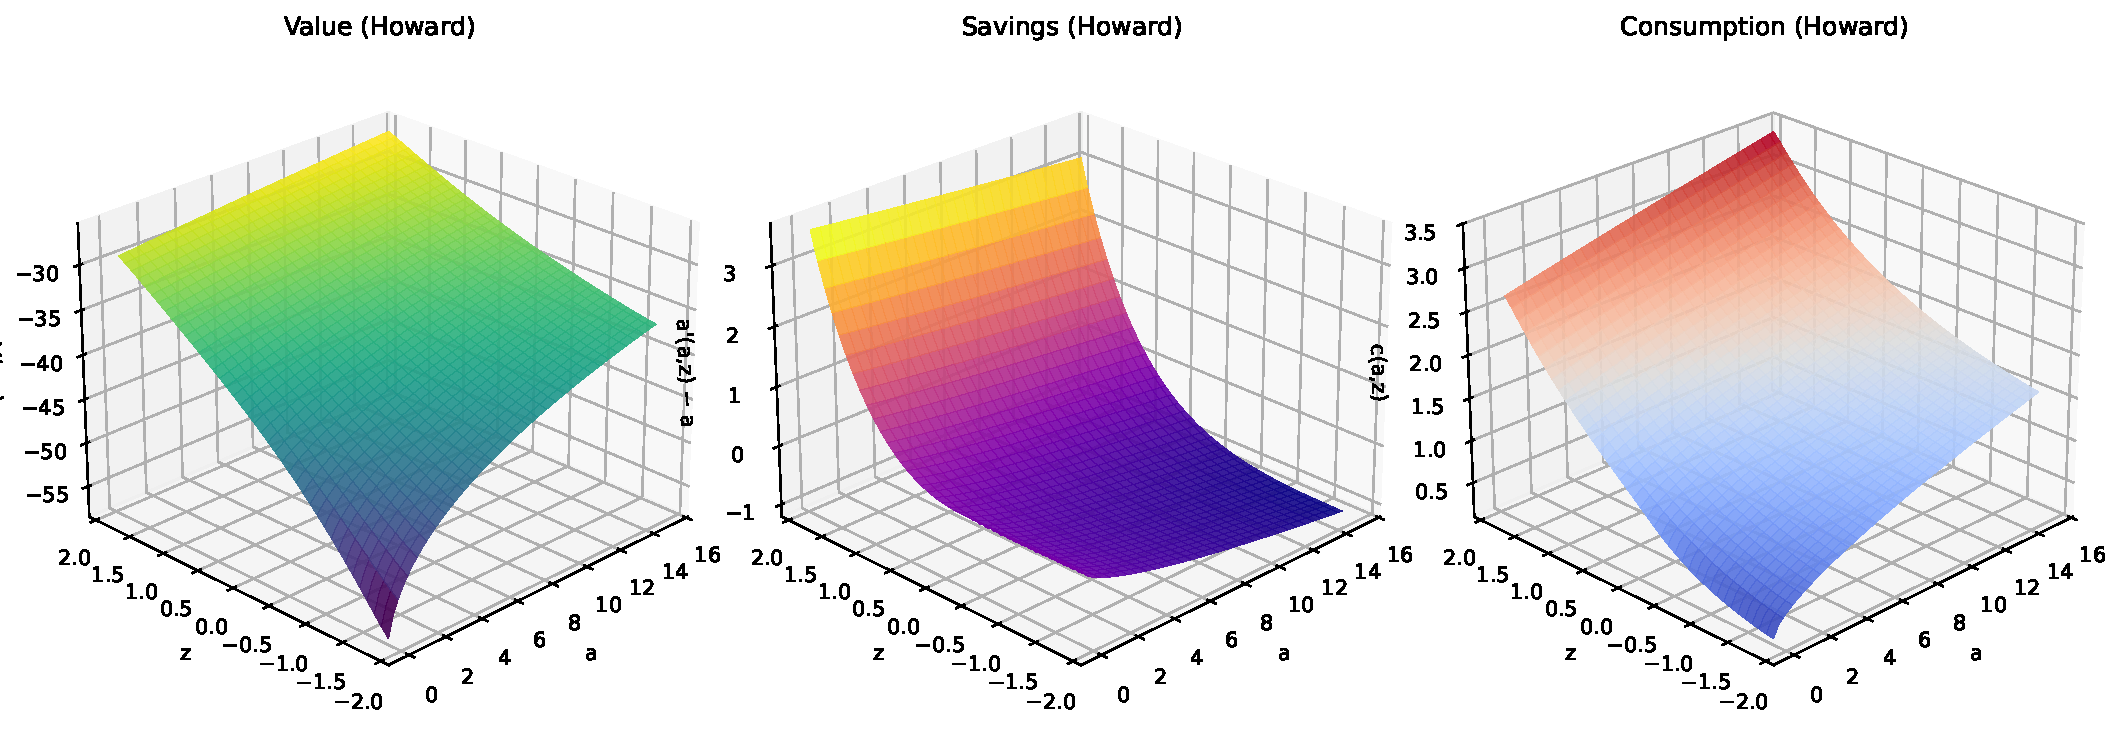
\includegraphics[width=0.92\textwidth]{fig_p2_3d_surfaces.pdf}
    \end{center}
    \vspace{-0.5em}
    \small
    \textbf{Left}: $V(a,z)$ concave in $a$, increasing and convex in $z$ (log-income curvature). \quad
    \textbf{Middle}: Net savings $a'(a,z)-a$ increasing in both $a$ and $z$; negative for low-$a$, low-$z$ agents (dis-savers at the constraint). \quad
    \textbf{Right}: Consumption $c(a,z)$ increasing and concave in $a$; agents with high $z$ consume a larger level but also a smaller fraction of resources.
\end{frame}

% ============================================================================
% SLIDE 11: P2 -- METHOD COMPARISON
% ============================================================================
\begin{frame}{Problem 2: Method Comparison at Selected $z$ Values}
    \vspace{-0.3em}
    \begin{center}
        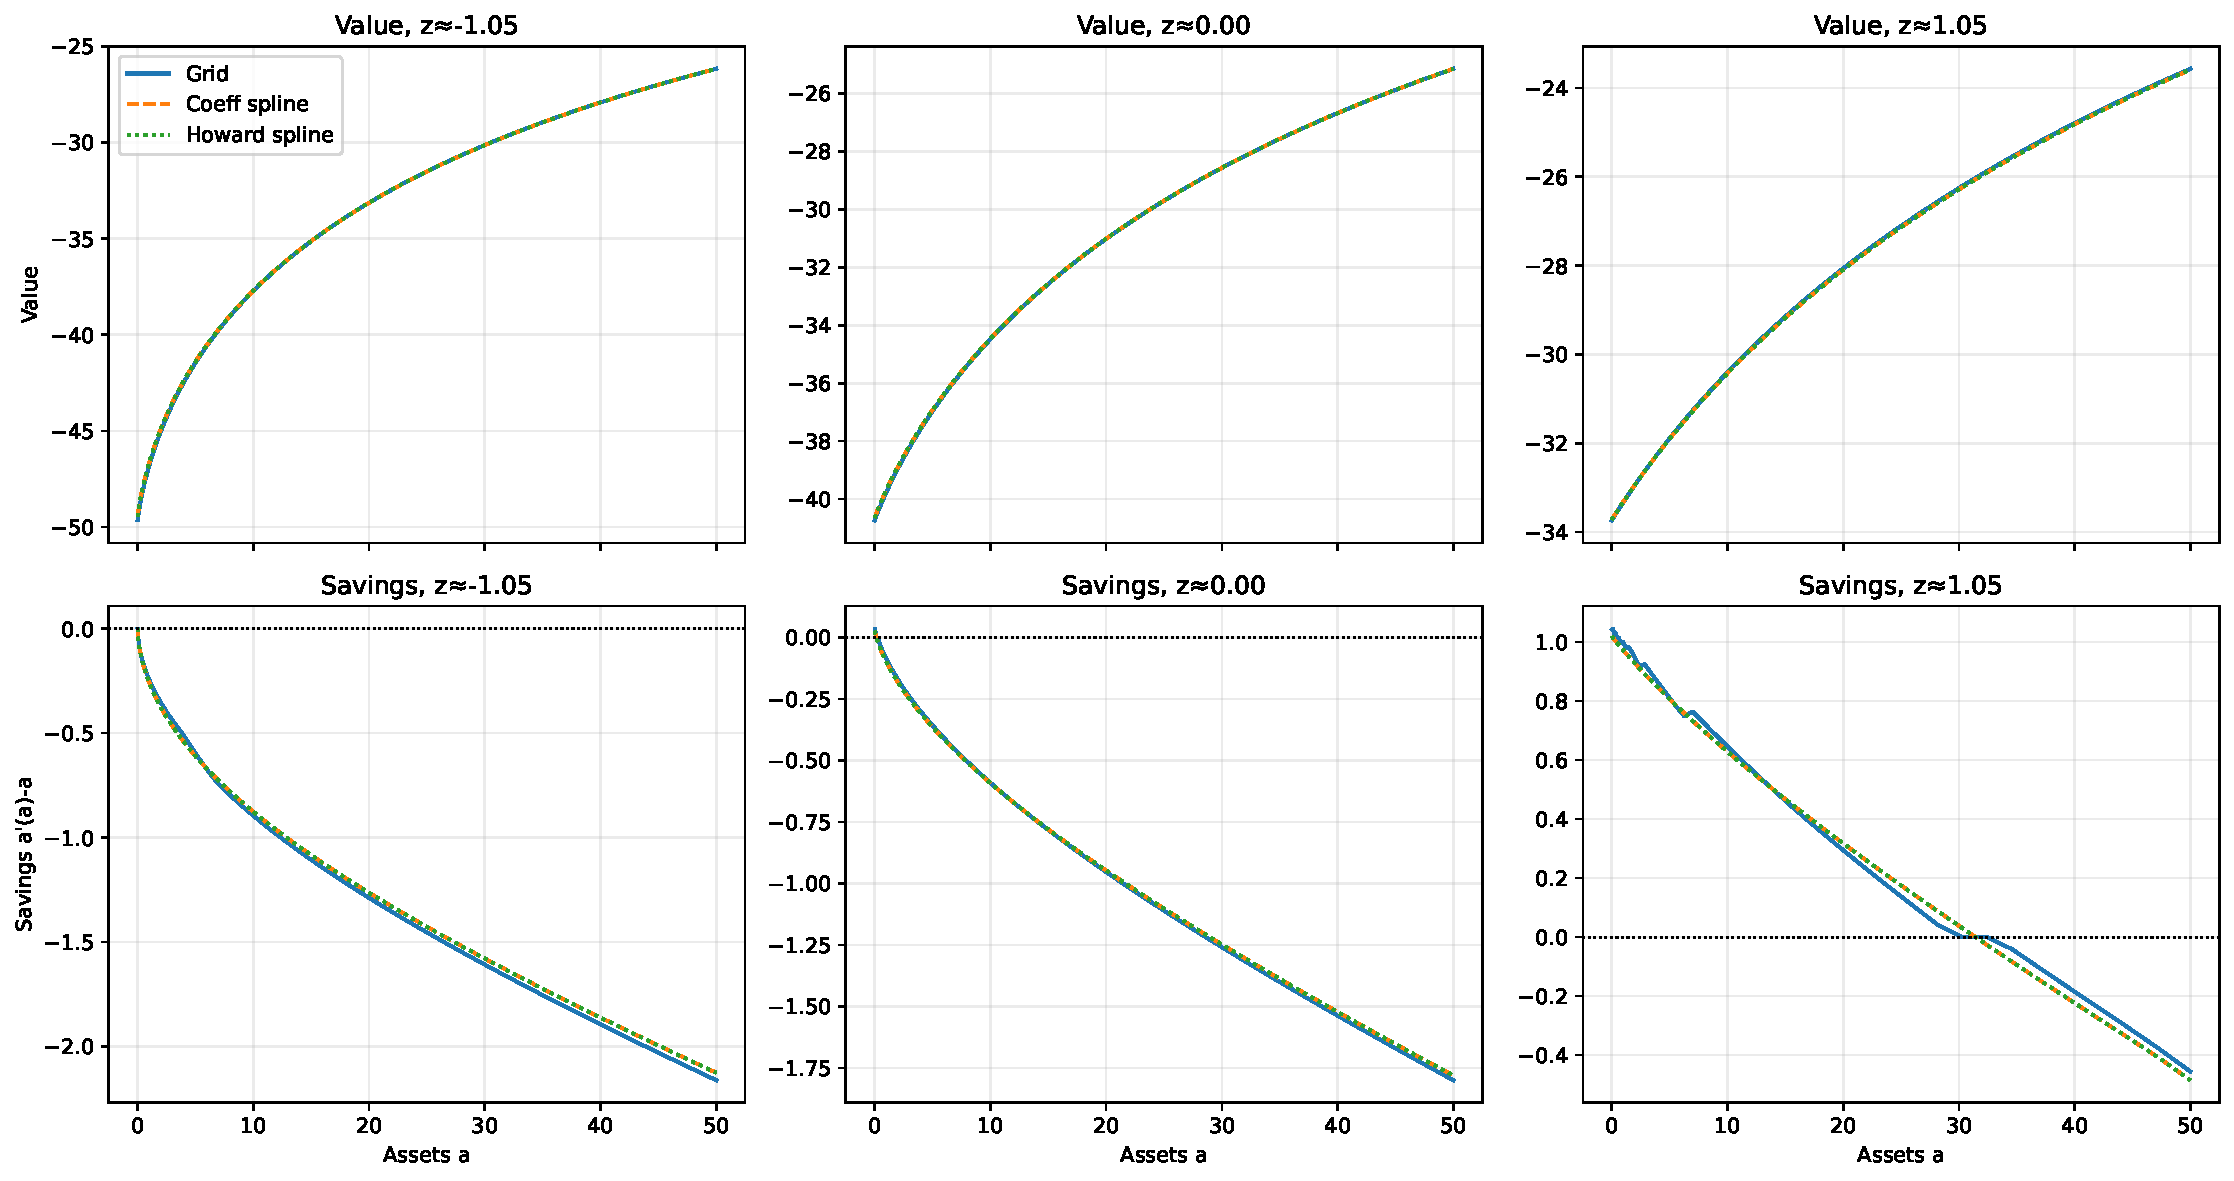
\includegraphics[width=0.92\textwidth]{fig_p2_method_comparison_full.pdf}
    \end{center}
    \vspace{-0.5em}
    \small
    \textbf{Top row}: value functions over full asset range $a\in[0,50]$; \textbf{Bottom row}: net savings $a'(a,z)-a$. Columns: $z \in \{-1, 0, 1\}$ (low, median, high income). All three methods (Grid VFI, Coeff spline, Howard spline) evaluated on the same VFI grid overlap tightly. Max absolute differences (interior): value $<10^{-4}$, savings $<10^{-3}$.
\end{frame}

% ============================================================================
% SLIDE 12: P2 -- DECISION RULES AND MPC
% ============================================================================
\begin{frame}{Problem 2: Decision Rules and Marginal Propensity to Consume}
    \vspace{-0.3em}
    \begin{center}
        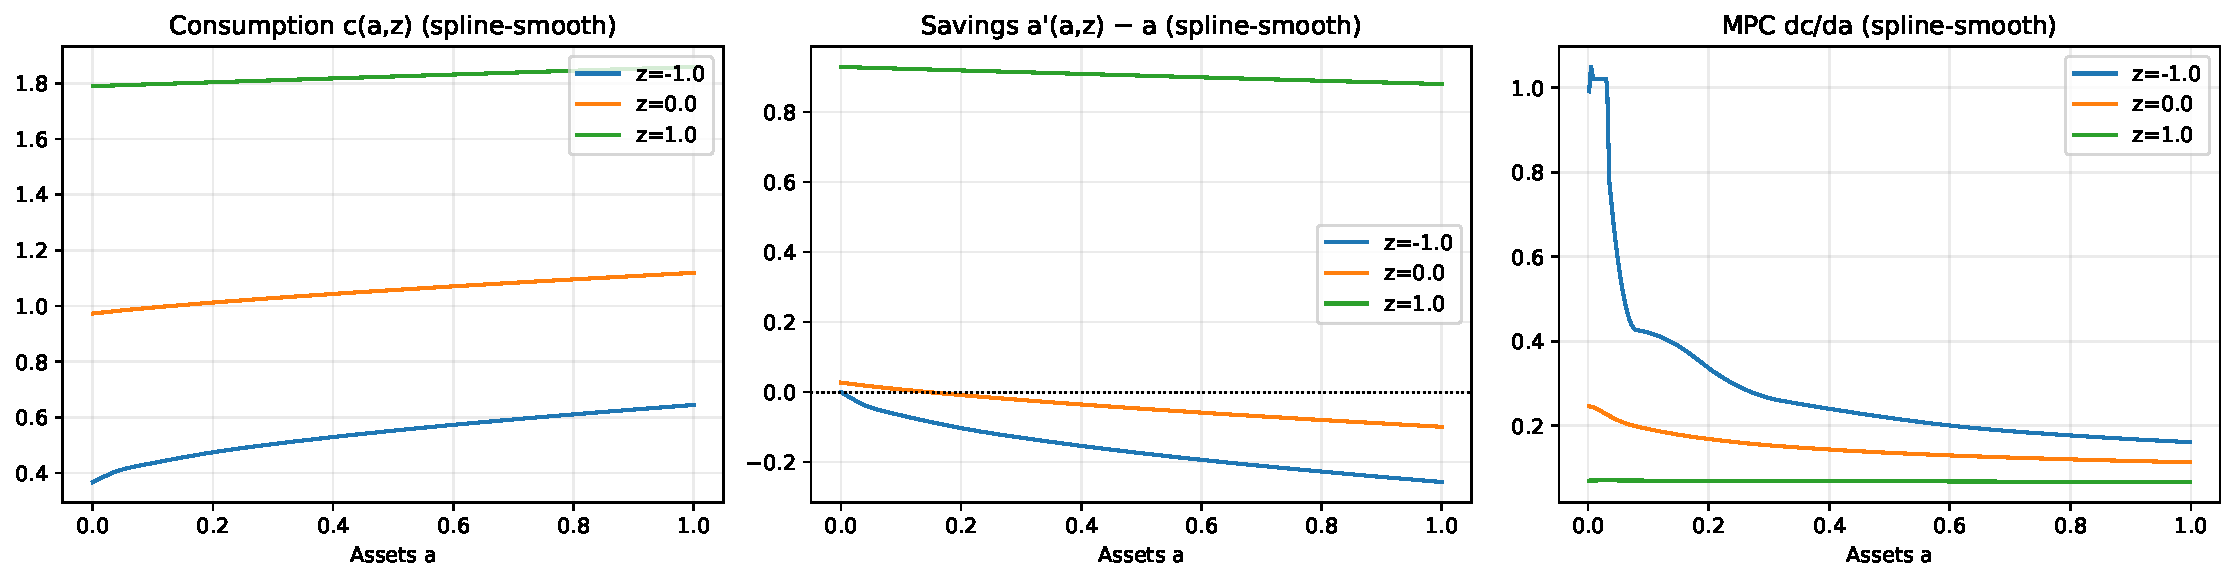
\includegraphics[width=0.92\textwidth]{fig_p2_decision_rules.pdf}
    \end{center}
    \vspace{-0.5em}
    \small
    Evaluated on $a\in[0,1]$ using the spline-smooth Howard solution. \textbf{Left}: Consumption increases with $a$ (concave) and with $z$ (richer and more productive agents consume more). \textbf{Middle}: Net savings cross zero at the precautionary buffer stock. \textbf{Right}: MPC is highest near the borrowing constraint and declines sharply --- a hallmark of hand-to-mouth behavior at low wealth.
\end{frame}

% ============================================================================
% SLIDE 13: P2 -- EULER EQUATION CHECK
% ============================================================================
\begin{frame}{Problem 2: Euler Equation Residuals}
    \vspace{-0.5em}
    \begin{columns}[T]
        \begin{column}{0.60\textwidth}
            \begin{center}
                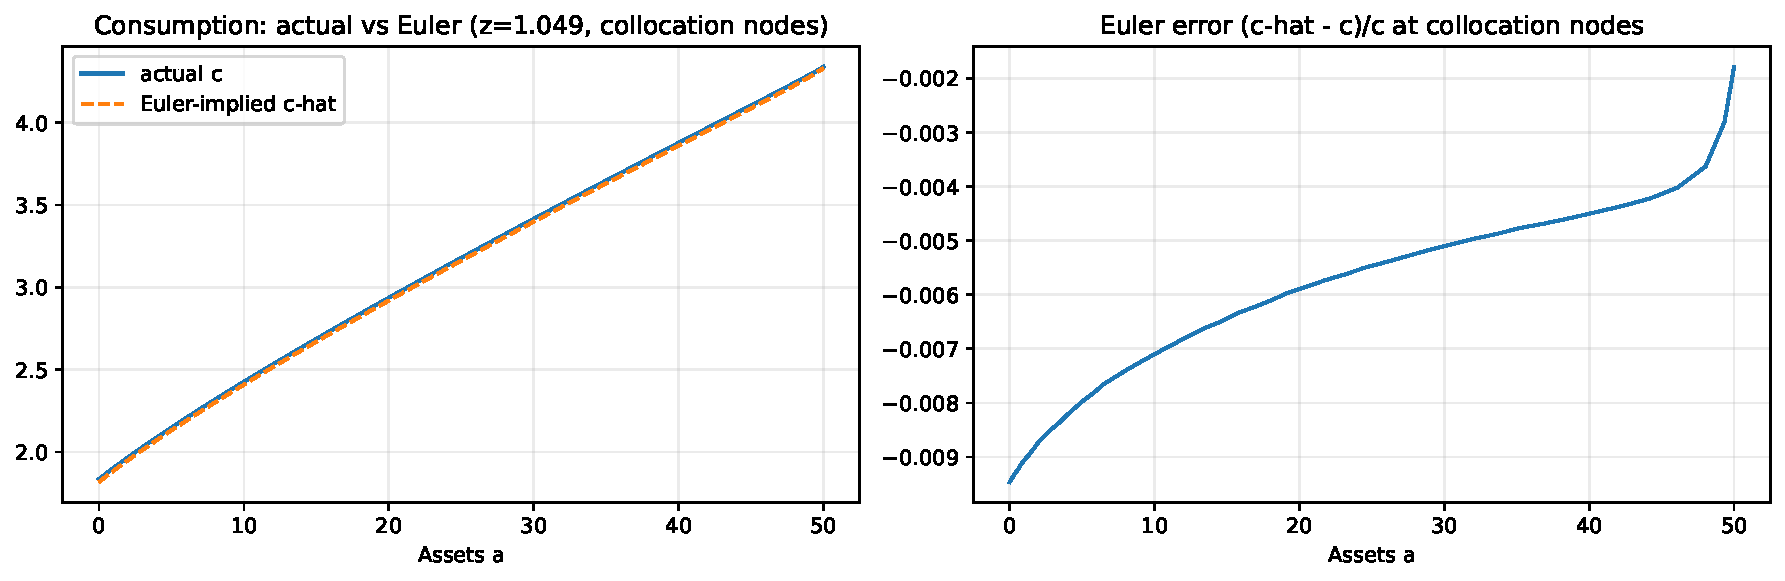
\includegraphics[width=\linewidth]{fig_p2_euler_check.pdf}
            \end{center}
        \end{column}
        \begin{column}{0.37\textwidth}
            \footnotesize
            \textbf{Unconstrained Euler condition}:
            \[
            c(a,z)^{-\alpha} = \beta(1+r)\,\E\bigl[c(a',z')^{-\alpha}\bigr]
            \]
            Define consumption-equivalent error:
            \[
            \hat{c}(a,z) = \bigl[\beta(1+r)\,\E c'^{-\alpha}\bigr]^{-1/\alpha}
            \]

            \vspace{0.3em}
            \textbf{Results (collocation nodes)}\\
            Max $|\hat{c}-c|/c$ on unconstrained: \texttt{2.3e-01}

            \vspace{0.3em}
            \begin{alertblock}{Interpretation}
                \small\sloppy Large Euler errors at the sparse solve-grid collapse on a denser output grid.\par
            \end{alertblock}
        \end{column}
    \end{columns}
\end{frame}

% ============================================================================
% SLIDE 14: P2 -- ERGODIC DISTRIBUTION
% ============================================================================
\begin{frame}{Problem 2: Ergodic Distribution}
    \vspace{-0.5em}
    \begin{columns}[T]
        \begin{column}{0.60\textwidth}
            \begin{center}
                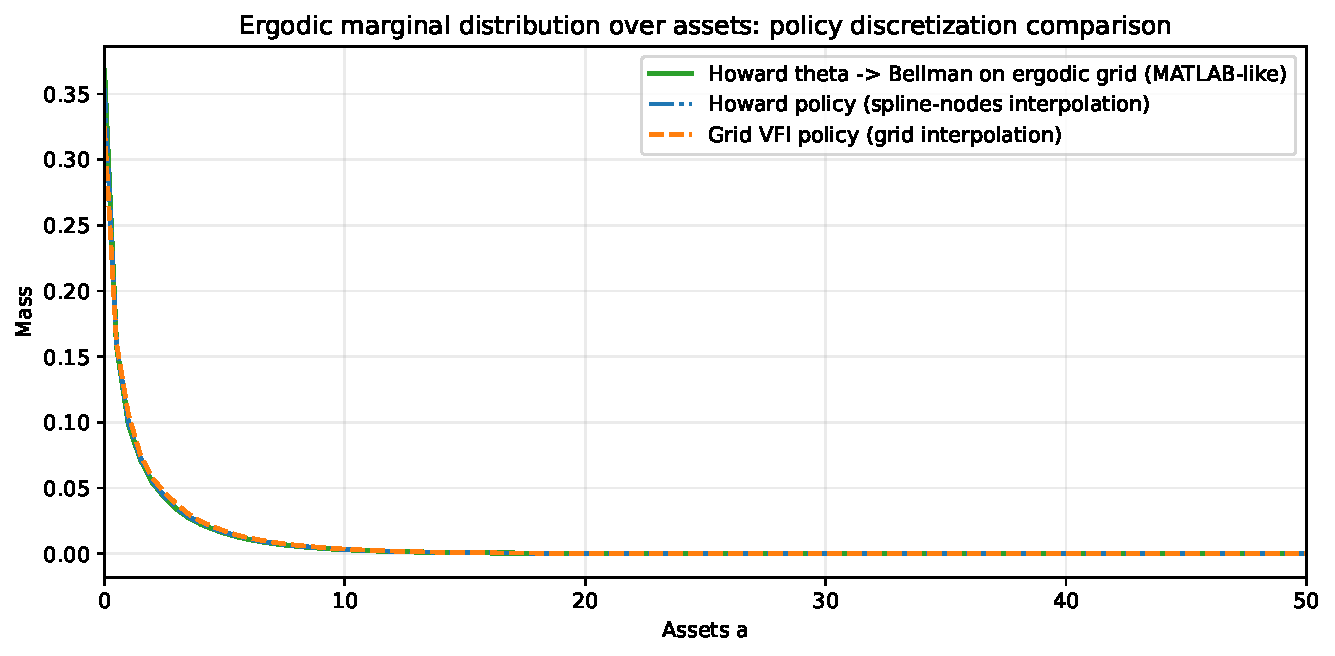
\includegraphics[width=\linewidth]{fig_p2_ergodic_dist.pdf}
            \end{center}
        \end{column}
        \begin{column}{0.37\textwidth}
            \footnotesize
            \textbf{Three policy discretization methods}:
            \begin{enumerate}\setlength\itemsep{0.15em}
                \item \textbf{theta$\to$Bellman}: recompute $a'(a,z)$ on ergodic grid from Howard $\theta$ (MATLAB-like)
                \item \textbf{Spline nodes}: interpolate Howard policy via spline
                \item \textbf{Grid VFI}: interpolate Grid-VFI policy
            \end{enumerate}

            \vspace{0.3em}
            \textbf{Aggregate moments}\\[0.2em]
            \renewcommand{\arraystretch}{1.1}
            \begin{tabular}{lc}
                \toprule
                & Howard \\
                \midrule
                Agg.\ assets & 1.72--1.89 \\
                Agg.\ income & 1.15 \\
                Agg.\ consump. & 1.15 \\
                Stationarity err & \texttt{3.5e-17} \\
                \bottomrule
            \end{tabular}

            \par\vspace{0.3em}
            {\sloppy\textbf{Note}: Moments differ across methods due to solve- vs.\ output-grid mismatch.\par}
        \end{column}
    \end{columns}
\end{frame}

% ============================================================================
% SLIDE 15: METHOD COMPARISON ACROSS PROBLEMS
% ============================================================================
\begin{frame}[shrink=8]{Method Comparison: Lessons from Both Problems}
    \vspace{-0.3em}
    \begin{adjustbox}{max width=\textwidth}
    \scriptsize
    \setlength{\tabcolsep}{5pt}
    \begin{tabular}{lp{3cm}p{3cm}p{3cm}}
        \toprule
        & \textbf{Grid VFI} & \textbf{Coeff VFI} & \textbf{Howard} \\
        \midrule
        Convergence & Slow ($300+$) & Slow (same) & Fast (6--7) \\
        Accuracy & Benchmark & $\approx$ Grid & $\approx$ Grid \\
        Solve grid & Dense grid & Greville nodes & Same \\
        Robustness & Robust & Basis-sensitive & Needs guess \\
        Wall time & 2.6\,s & 45\,s & $<$1\,s \\
        \bottomrule
    \end{tabular}
    \end{adjustbox}

    \vspace{0.2em}
    \begin{alertblock}{Main lesson}
        {\sloppy Howard acceleration reduces Bellman maximizations to single digits while preserving full coefficient-based accuracy.\par}
    \end{alertblock}
\end{frame}

% ============================================================================
% SLIDE 16: DIAGNOSTICS CHECKLIST
% ============================================================================
\begin{frame}{Diagnostics: What to Check After Solving}
    \begin{columns}[T]
        \begin{column}{0.48\textwidth}
            \small\textbf{Solution quality}
            \begin{enumerate}\setlength\itemsep{0.1em}
                \item \textbf{Bellman residual}: $\|V^{t+1}-V^t\|$ at convergence
                \item \textbf{Cross-check}: Grid VFI vs Howard on a dense evaluation grid
                \item \textbf{Policy monotonicity}: $a'(a)$ non-decreasing in $a$
                \item \textbf{Boundary}: $c = y + (1+r)a$ at the constraint
            \end{enumerate}
        \end{column}
        \begin{column}{0.48\textwidth}
            \small\textbf{Distribution quality}
            \begin{enumerate}\setlength\itemsep{0.1em}
                \item \textbf{Stationarity}: $\|n - nQ\|$ (P1: \texttt{1.3e-17}; P2: \texttt{3.5e-17})
                \item \textbf{Row-sum of $Q$}: each row $= 1$
                \item \textbf{Euler residual}: on dense output grid
                \item \textbf{Mass at boundary}: $a_{\max}$ should not be binding
            \end{enumerate}
        \end{column}
    \end{columns}

    \vspace{0.2em}
    \begin{block}{Rule of thumb}
        Convergence is \textit{necessary} but not \textit{sufficient}. Always verify residuals and moments.
    \end{block}
\end{frame}

% ============================================================================
% SLIDE 17: SUMMARY
% ============================================================================
\begin{frame}{Summary and Takeaways}
    \begin{columns}[T]
        \begin{column}{0.48\textwidth}
            \textbf{Problem 1 (discrete income)}
            \begin{itemize}\setlength\itemsep{0.2em}
                \item Howard converges in 7 iterations vs.\ 336 (Grid VFI) and 420 (Coeff VFI) --- same fixed point
                \item Unemployed agents hold less wealth; distribution mass concentrated at low $a$
                \item Stationarity check passes at machine precision
            \end{itemize}
        \end{column}
        \begin{column}{0.48\textwidth}
            \textbf{Problem 2 (continuous AR(1))}
            \begin{itemize}\setlength\itemsep{0.2em}
                \item Greville collocation nodes $\ne$ output grid; always re-evaluate on uniform grid before computing moments
                \item MPC decreasing in $a$: hand-to-mouth behavior at the borrowing constraint
                \item Euler errors on the sparse solve grid are misleading --- use a dense output grid for residual reporting
            \end{itemize}
        \end{column}
    \end{columns}

    \vspace{0.5em}
    \centering
    \small
    Code: \texttt{examples/pset3/notebooks/pset3\_problem1.ipynb} and \texttt{pset3\_problem2.ipynb}
\end{frame}

% ============================================================================
% APPENDIX
% ============================================================================
\appendix

\begin{frame}[plain]
    \begin{center}
        {\Large \textbf{Appendix}}
    \end{center}
\end{frame}

% ============================================================================
% APPENDIX A: CALIBRATION TABLES
% ============================================================================
\begin{frame}{Appendix: Calibration}
    \footnotesize
    \begin{columns}[T]
        \begin{column}{0.47\textwidth}
            \textbf{Problem 1: Two-State Income}\\[0.3em]
            \renewcommand{\arraystretch}{1.1}
            \begin{tabular}{llc}
                \toprule
                \textbf{Symbol} & \textbf{Description} & \textbf{Value} \\
                \midrule
                $\beta$ & Discount factor & 0.95 \\
                $r$ & Interest rate & 0.04 \\
                $b$ & Unemployment income & 0.25 \\
                $\sigma$ & Job-loss rate & 0.10 \\
                $\lambda$ & Job-finding rate & 0.25 \\
                $a_{\max}$ & Asset upper bound & 10 \\
                $n_{\text{breaks}}$ & Spline breakpoints & 51 \\
                $n_{\text{nodes}}$ & Greville nodes & 53 \\
                $K$ & Distribution grid & 551 \\
                \bottomrule
            \end{tabular}
        \end{column}
        \begin{column}{0.47\textwidth}
            \textbf{Problem 2: AR(1) Income}\\[0.3em]
            \renewcommand{\arraystretch}{1.1}
            \begin{tabular}{llc}
                \toprule
                \textbf{Symbol} & \textbf{Description} & \textbf{Value} \\
                \midrule
                $\beta$ & Discount factor & 0.95 \\
                $r$ & Interest rate & 0.02 \\
                $\alpha$ & CRRA coefficient & 1.5 \\
                $\rho$ & AR(1) persistence & 0.90 \\
                $\sigma$ & AR(1) innovation std.\ dev. & 0.20 \\
                $k$ & Quadrature nodes & 7 \\
                $a_{\max}$ & Asset upper bound & 50 \\
                $n_a$ & Asset breakpoints & 51 \\
                $n_z$ & Income breakpoints & 15 \\
                \bottomrule
            \end{tabular}
        \end{column}
    \end{columns}
\end{frame}

% ============================================================================
% APPENDIX B: HOWARD LINEAR SYSTEM
% ============================================================================
\begin{frame}{Appendix: Howard Improvement --- Linear System (Problem 1)}
    \small
    With fixed policy $a'_e(a)$ and $a'_u(a)$, the value functions satisfy:
    \[
    \footnotesize
    \begin{pmatrix}
    \Phi - \beta(1{-}\sigma)\Phi(a'_e) & -\beta\sigma\Phi(a'_u) \\
    -\beta\lambda\Phi(a'_e) & \Phi - \beta(1{-}\lambda)\Phi(a'_u)
    \end{pmatrix}
    \begin{pmatrix}
    \theta_e \\ \theta_u
    \end{pmatrix}
    =
    \begin{pmatrix}
    u(c_e) \\ u(c_u)
    \end{pmatrix}
    \]
    where $\Phi = \Phi(a_{\text{nodes}})$ is the $K\!\times\!K$ basis matrix and $\Phi(a'_e)$ evaluates the basis at policy $a'_e(a_{\text{nodes}})$.

    \vspace{0.4em}
    \textbf{For Problem 2} (single state variable $z$, 901 collocation nodes):
    \[
    \bigl[\Phi - \beta\textstyle\sum_{k=1}^K w_k \Phi(a'(\cdot),\,\rho z + \sigma\varepsilon_k)\bigr]\,\theta = u(c)
    \]
    where $\Phi(a',z')$ is the 901$\times$901 tensor-product basis matrix evaluated at next-period states.

    \vspace{0.3em}
    \begin{block}{Computational note}
        Both systems are \textbf{dense} and solved by LU factorization. Problem 1: $1102\!\times\!1102$ block; Problem 2: $901\!\times\!901$. This motivates using iterative policy updates rather than forming the full matrix at every step.
    \end{block}
\end{frame}

\end{document}
